\levelstay{Noncommensurate Frequencies}

\leveldown{Power in an exponential}

So far we've only talked about signals that are periodic in the time that we measure, ie. we've dealt with sinusoids of the form $\exp\left(2\pi nq/N\right)$. What happens if we have a sinusoid at an arbitrary frequency that is not one of the Fourier frequencies? To get an idea let's compute the Fourier series for a noncommensurate exponential, $\exp\left(i2\pi\xi x\right)$
\begin{align*}
f_{k} & = \int_{0}^{1}e^{-i2\pi kx}e^{i2\pi\xi x}\, dx\\
f_{k} & = \frac{\exp\left(i2\pi(\xi-k)\right)-1}{i2\pi(\xi-k)}\\
f_{k} & = \exp\left(i2\pi(\xi-k)/2\right)\frac{e^{i2\pi(\xi-k)/2}-e^{-i2\pi(\xi-k)/2}}{i2\pi(\xi-k)}\\
f_{k} & = \exp\left(i2\pi(\xi-k)/2\right)\textrm{sinc}\left(\xi-k\right)\\
|f_{k}|^{2} & = \textrm{sinc}^{2}\left(\xi-k\right)
\end{align*}
where $\textrm{sinc}(x)=\sin\left(\pi x\right)/\pi x$. To understand what this means, start by considering what happens if $\xi$ is an integer. If $\xi$ is an integer then $\exp\left(i2\pi\xi x\right)$ is commensurate on $[0,1]$ and the Fourier series has only one nonzero term, since the sinc function is zero for all integer arguments except 0. Therefore, in the case $f_{k}=\delta_{k,\xi}$. However, if $\xi$ is not an integer then the Fourier series is nonzero for all $k$.

The case of a DFT essentially the same thing happens. Let's see this explicitly by computing the DFT, \footnote{To compute the finite sum we use the formula $1+x+x^{2}+\cdots+x^{N-1}=(x^{N}-1)/(x-1)$.}
\begin{align*}
X(k) & = \sum_{n=0}^{N-1}e^{-i2\pi nk/N}e^{i2\pi n\xi/N}\quad\xi\textrm{ not an integer}\\
X(k) & = \sum_{n=0}^{N-1}\left[e^{i2\pi(\xi-k)/N}\right]^{n}\\
X(k) & = \frac{\exp\left[i2\pi\left(\xi-k\right)\right]-1}{\exp\left[i2\pi\left(\xi-k\right)/N\right]-1}\\
X(k) & = e^{i\pi(\xi-k)(N-1)/N}\frac{\sin\left(\pi\left(\xi-k\right)\right)}{\sin\left(\pi\left(\xi-k\right)/N\right)}\\
|X(k)|^{2} & = \left(\frac{\sin\left[\pi\left(\xi-k\right)\right]}{\sin\left[\pi\left(\xi-k\right)/N\right]}\right)^{2}
\end{align*}
This says that the power is spread out over several values of $k$ just like in the Fourier series case. In Figure 1 we show the numerically computed $|\textrm{DFT}|^2$ of a noncommensurate exponential along with the expected curve.


\quickfig{\columnwidth}{leakage.pdf}
{Numerically computed DFT (power) of a noncommensurate exponential
with theory curve. The signal is $\exp\left[i2\pi n\xi/N\right]$
with $N=20$ and $\xi=12.2$. The mod square of the DFT is shown in
blue and the theory curve is in red.}
{Flo:leakage}


\levelstay{Power in sinusoids}

\leveldown{Fourier Series}

Consider a signal over a finite interval given by $s(x)=\cos(2\pi\xi x)$
where $x\in[0,1]$. Note that $\nu$ is the number of oscillations
of the signal over the sampled interval. The power in this signal
is \begin{eqnarray*}
P & = & \int_{0}^{1}s(t)^{2}dx\\
P & = & \int_{0}^{1}\cos(2\pi\xi x)^{2}dx\\
P & = & \frac{1}{2}\left[1+\textrm{sinc}\left(4\xi\right)\right]\end{eqnarray*}
This curve is plotted in Figure \ref{Flo:PowerFromNoncommensurateSinusoid}.

%
\begin{figure}
\begin{centering}
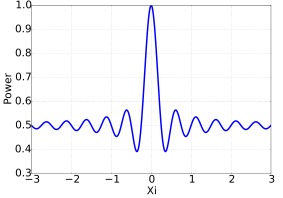
\includegraphics[width=8cm]{power.pdf}
\par\end{centering}

\caption{Measured power in a sinusoid with $\xi$ cycles over the measurement
time. Note that away from DC the power is nearly $1/2$ as appropriate
for an infinitely long sinusoid. Note also that commensurate sinewaves
give exactly $1/2$.}


\label{Flo:PowerFromNoncommensurateSinusoid}
\end{figure}


It would be nice to see explicitly that this strange power curve is
reproduced in frequency space. To do this, we will compute the Fourier
Series for the signal, and then sum the squares of the Fourier coefficients
to see if we get this same total power. The Fourier coefficients for
the sinusoid are computed easily because we already worked them out
for exponentials,\begin{align*}
s(t) & = \cos(2\pi\xi x)\\
s(t) & = \frac{1}{2}\left[e^{i2\pi\xi x}+e^{-i2\pi\xi x}\right]\\
s_{k} & = \frac{1}{2}\left[e^{i\pi(\xi-k)}\textrm{sinc}\left(\xi-k\right)+e^{-i\pi(\xi+k)}\textrm{sinc}\left(\xi+k\right)\right]\\
|s_{k}|^{2} & = \frac{1}{4}\left[\textrm{sinc}\left(\xi-k\right)^{2}+\textrm{sinc}\left(\xi+k\right)^{2}+\right.\\
 & + \left.2\cos\left(2\pi\xi\right)\textrm{sinc}\left(\xi-k\right)\textrm{sinc}\left(\xi+k\right)\right]
\end{align*}
The total power should be $\sum_{k=-\infty}^{\infty}|s_{k}|^{2}$,
so to check for consistency we need to do the sum over $k$. The necessary
sums are done explicitly in appendix ??, and the result is that\[
\sum_{k=-\infty}^{\infty}|s_{k}|^{2}=\frac{1}{2}\left[1+\textrm{sinc}\left(4\xi\right)\right]\]
in agreement with the time domain integral. This is an important result.
It means that 


\levelstay{DFT}

Frequently one wants to determine the amount of power at each frequency
in an experimentally obtained time series. To find out how to get
this, let's consider a cosine wave\[
s(t)=A\cos\left(2\pi ft\right)\]
 The power in this signal is $A^{2}/2$. What happens when we sample
the signal and compute the DFT? The sampled signal can be written
as\begin{eqnarray*}
s(n) & = & A\cos\left(2\pi fn\cdot\delta t\right)\\
s(n) & = & \frac{A}{2}\left[\exp\left(i2\pi fn\cdot\delta t\right)+\exp\left(-i2\pi fn\cdot\delta t\right)\right]\end{eqnarray*}
 where $\delta t$ is the sampling interval. Noting that $f\cdot\delta t=\xi/N$
we can take the DFT\begin{align*}
s_{k} & = \frac{A}{2}e^{-i\pi k(N-1)/N}\left[e^{i\pi\xi(N-1)/N}\frac{\sin\left[\pi\left(\xi-k\right)\right]}{\sin\left[\pi\left(\xi-k\right)/N\right]}+\right.\\
 & + \left.e^{-i\pi\xi(N-1)/N}\frac{\sin\left[\pi\left(\xi+k\right)\right]}{\sin\left[\pi\left(\xi+k\right)/N\right]}\right]\\
s_{k} & = \left(\frac{A}{2}\right)^{2}\left[\left(\frac{\sin\left[\pi\left(\xi-k\right)\right]}{\sin\left[\pi\left(\xi-k\right)/N\right]}\right)^{2}+\right.\\
 & + \left.\left(\frac{\sin\left[\pi\left(-\xi-k\right)\right]}{\sin\left[\pi\left(-\xi-k\right)/N\right]}\right)^{2}+\right]\\
|s_{k}|^{2} & = \frac{A^{2}}{4}\left[\frac{\sin\left[\pi\left(\xi-k\right)\right]}{\sin\left[\pi\left(\xi-k\right)/N\right]}+\frac{\sin\left[\pi\left(-\xi-k\right)\right]}{\sin\left[\pi\left(-\xi-k\right)/N\right]}\right]^{2}
\end{align*}



